% Copyright (c) 2020, Santtu Söderholm <santtu.soderholm@tuni.fi>
%
% This file may be distributed and/or modified under the LaTeX Project Public License.
%
\def\checkmark{\tikz\fill[scale=0.4](0,.35) -- (.25,0) -- (1,.7) -- (.25,.15) -- cycle;}
\def\scalecheck{\resizebox{\widthof{\checkmark}*\ratio{\widthof{x}}{\widthof{\normalsize x}}}{!}{\checkmark}}

\begin{frame}[noframenumbering, plain]
\titlepage
\end{frame}


\begin{frame}[noframenumbering, plain]{Table of contents}
\tableofcontents
\end{frame}
\section{Headsail}
\begin{frame}{SoC Hub Headsail}
  \begin{itemize}
          \item \textbf{RISC-V} based \textbf{SoC} developed at Tampere University
          \item 4-core multicore based on with 64-bit CVA6~\cite{zaruba2019costCVA6} cores called HPC
          \item Deep Learning Accelerator (\textbf{DLA}) for CNNs
          \item Large SDRAM (128MB)
  \end{itemize}
  \vfill
  \textbf{Goal 1:} Model Headsail and the DLA as a virtual platform
\end{frame}

\section{DLA}
\begin{frame}{DLA}
    \begin{columns}
        \begin{column}{0.4\textwidth}
          \begin{itemize}
                  \item Supported operations are \textbf{Conv2D}, \textbf{Bias} and \textbf{ReLU}
                  \item Convolution performed by 16x16 MAC array
                  \item Optional \textbf{post-processing} pipeline for Bias and ReLU
                  \item Arithmetic width of 16 bits, results 8 bits signed
                  \item Operation parameters defined in register interface
          \end{itemize}
        \end{column}
        \begin{column}{0.6\textwidth}
            \begin{figure}
                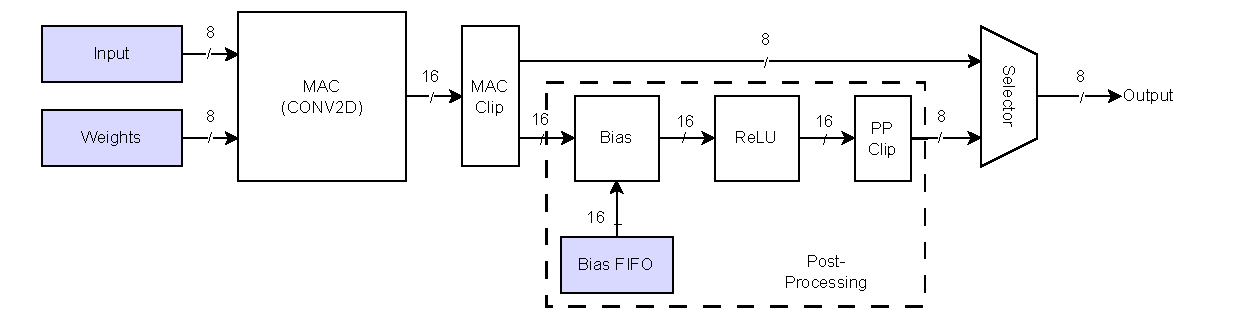
\includegraphics[width=1.0\textwidth]{../../thesis/img/dla-internal.pdf}
                \caption{DLA's high-level architecture}
            \end{figure}
        \end{column}
    \end{columns}
    \vfill
  \textbf{Goal 2:} Build software stack for the DLA to run inference on arbitrary convolutional models
\end{frame}

\begin{frame}{DLA}
\begin{columns}
    \begin{column}{0.5\textwidth}
        \begin{itemize}
                \item \textbf{HPC} (RV64) controls DLA with the register interface
                \item DLA internal databanks filled with data from \textbf{SDRAM}
                \item 64 and 32-bit AXI buses enable fast data transfers
                \item DLA writes results to data banks or directly back to SDRAM
        \end{itemize}
      \end{column}
    \begin{column}{0.5\textwidth}
  \begin{figure}
    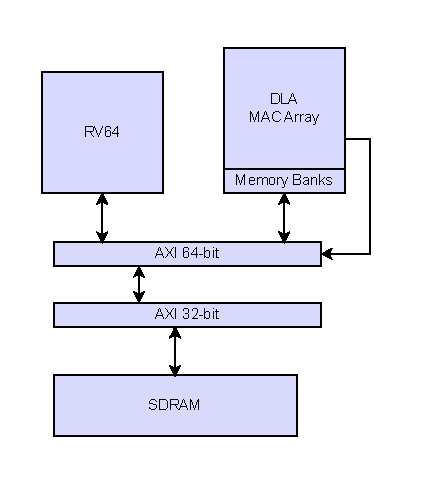
\includegraphics[width=0.7\textwidth]{../../thesis/img/dla-setup.drawio.pdf}
    \caption{DLA's integration to the SoC}
  \end{figure}
    \end{column}
\end{columns}
\end{frame}

\section{Components needed for inference}
\begin{frame}{Components needed for inference}
\begin{table}[ht]
\centering
\caption{System Configuration and Components}
\begin{tabular}{|l|p{8cm}|}
\hline
\textbf{Item} & \textbf{Description} \\ \hline
Platform & SocHub's Headsail SoC with a Deep Learning Accelerator. Development done in a virtual prototype. \\ \hline
Compiler & riscv64-unknown-none-elf. \\ \hline
BSP (Board Support Package) & Support for necessary hardware peripherals. \\ \hline
Machine Learning Compiler & Convert high-level models to Headsail compatible code. \\ \hline
Model & 4 MLPerf Tiny reference models \\ \hline
Validation dataset &  4 datasets defined by MLPerf Tiny benchmark  \\ \hline
\end{tabular}
\label{tab:system_components}
\end{table}
\end{frame}

\section{Virtual Prototype}
\begin{frame}{Virtual Prototype}
  \begin{itemize}
    \item Virtual prototype made in \textbf{Renode}: High-level full system emulator
    \item Offers large catalogue of known processors and ability to implement non-unified memory maps, with overlapping addresses for each processor
    \item Headsail DLA's virtual prototype developed with Renode's Python Peripheral API
    \item Prototype models Headsail's complete memory map and the CPUs
  \end{itemize}
\end{frame}

\section{TVM}
\begin{frame}{TVM}
  \begin{itemize}
          \item Open-source Machine Learning Compiler that supports large variety of hardware backends~\cite{TVM}
          \item \textbf{BYOC API} offers a way to integrate custom accelerators to \textbf{TVM}
          \item Runtime for bare-metal targets via microTVM, dependent only on C standard library
          \item Custom legalization pass performs graph transformation to support custom hardware targets
  \end{itemize}
\end{frame}

\section{Board Support Package}
\begin{frame}{Board Support Package}
  \begin{itemize}
    \item Small \textbf{BSP} written in Rust, with \texttt{riscv-rt}~\cite{riscv_rt} for runtime
    \item SoC initialization code provided with \textsc{init-hpc} program
    \item Includes driver for the DLA with high-level operator API
    \item \textbf{FFI} generated with \texttt{cbindgen} to provide C bindings
  \end{itemize}
\end{frame}


\section{MLPerf Tiny}
\begin{frame}{MLPerf Tiny}
\begin{table}[ht]
\centering
\caption{Tiny Performance Benchmarks, from~\parencite{tinyperf}}
\begin{adjustbox}{max width=\textwidth}
\begin{tabular}{lccc}
  \toprule
  \textbf{Benchmark} & \textbf{Dataset (Input Size)} & \textbf{Model (TFLite Model Size)} & \textbf{Quality Target (Metric)} \\
  \midrule
  Keyword Spotting & Speech Commands (49x10) & DS-CNN (52.5 KB) & 90\% (Top-1) \\
  Visual Wake Words & VWW Dataset (96x96)  & MobileNetV1 (325 KB) & 80\% (Top-1) \\
  Image Classification & CIFAR10 (32x32) & ResNet (96 KB) & 85\% (Top-1) \\
  Anomaly Detection & ToyADMOS (5x128)  & FC-AutoEncoder (270 KB) & .85 (AUC) \\
  \bottomrule
\end{tabular}
\end{adjustbox}
\label{tab:tinyperf}
\end{table}
\begin{itemize}
        \centering
        \item \textbf{Inference} benchmark for embedded devices that models real-life use cases
        \item Offers pretrained \textbf{quantized} reference network as TFlite models
\end{itemize}
\end{frame}

\section{Software Architecture}
\begin{frame}{Final Software Architecture}
  \begin{columns}
    \begin{column}{0.3\textwidth}
      \begin{itemize}
        \item Rust-based BSP with C-bindings
        \item C support with GCC and Newlib
        \item \textbf{TVM} codegen for target
        \item Flashed with JTAG -> OpenOCD -> GDB stack
        \item Benchmark host to target communication with UART
        \item \textbf{MLPerf Tiny} as use case
      \end{itemize}
    \end{column}
    \begin{column}{0.7\textwidth}
        \begin{figure}
          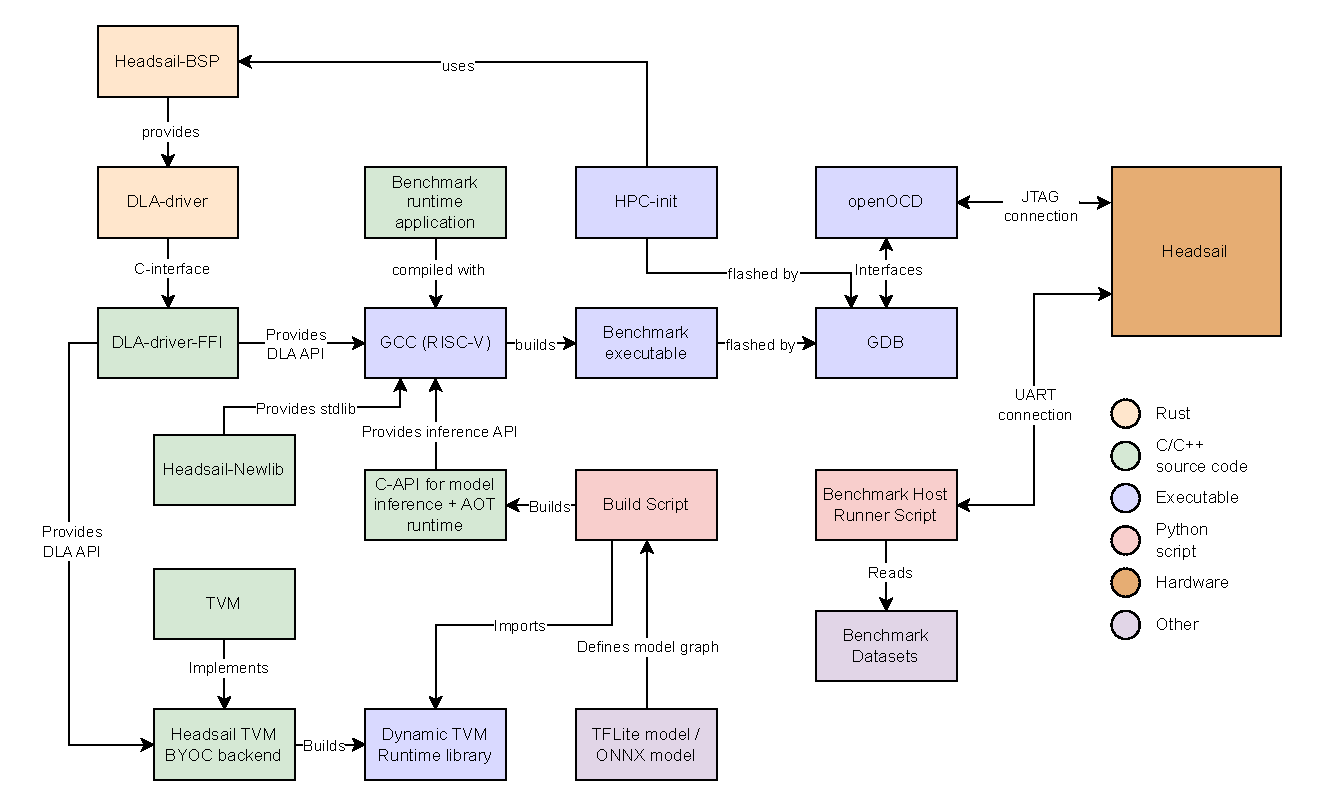
\includegraphics[height=0.6\textheight]{../../thesis/img/dla-architecture-new.pdf}
          \caption{Projects software architecture}
        \end{figure}
      \end{column}
  \end{columns}
\end{frame}

\section{Results}
\begin{frame}{Results}
\begin{table}[h]
\centering
\caption{MLPerf Tiny benchmark results for HPC and HPC with DLA.}
\begin{tabular}{|l|l|c|c|c|c|}
\hline
  \multirow{2}{*}{\textbf{Task}}  & \multirow{2}{*}{\textbf{Target}}  & \multirow{2}{*}{\textbf{Accuracy}} & \multirow{2}{*}{\textbf{Precision}} & \multirow{2}{*}{\textbf{Recall}} & \multirow{2}{*}{\shortstack[c]{\textbf{Passes}\\ \textbf{MLPerf Tiny}}} \\
  & & & & & \\\hline
\multirow{2}{*}{\shortstack[l]{\textbf{Keyword}\\ \textbf{Spotting (KWS)}}}
                                  & \textbf{HPC} & 0.90               & 0.92       & 0.90     & \scalecheck                          \\ \cline{2-6}
                                  & \textbf{HPC+DLA} & 0.90               & 0.92   & 0.90         & \scalecheck                          \\ \hline
\multirow{2}{*}{\shortstack[l]{\textbf{Image}\\ \textbf{Classifcation (IC)}}}
                                  & \textbf{HPC} & 0.88               & 0.88      & 0.88      & \scalecheck                          \\ \cline{2-6}
                                  & \textbf{HPC+DLA} & 0.69               & 0.74      & 0.70      &                            \\ \hline
\multirow{2}{*}{\shortstack[l]{\textbf{Visual Wake}\\ \textbf{Words (VWW)}}}
                                  & \textbf{HPC} & 0.83               & 0.83        & 0.84    & \scalecheck                          \\ \cline{2-6}
                                  & \textbf{HPC+DLA} & 0.50               & 0.50   & 0.50          &                            \\ \hline
\multirow{2}{*}{\shortstack[l]{\textbf{Anomaly}\\ \textbf{Detection (AD)}}}
                                  & \textbf{HPC } & \multicolumn{3}{c|}{\textbf{AUC} = 0.68}     &   \\ \cline{2-6}
                                  & \textbf{HPC+DLA} & \multicolumn{3}{c|}{-}      &                            \\ \hline

\end{tabular}
\label{tab:benchmark-results}
\end{table}
\begin{itemize}
  \centering
  \item Conclusion: \textbf{DLA-vp} doesn't have full compatibility with MLPerf Tiny \textbf{reference} models
  \item Solution: \textbf{Custom} build models and training flow to attain accurate models
\end{itemize}

\end{frame}
\section{References}

\begin{frame}{References}
    \printbibliography[heading=none]
\end{frame}

\finalpage{Thank you for listening!}{Questions?}
